\documentclass[]{beamer}
\usetheme{Dresden}
% \useoutertheme{split}

\usepackage{color}
\usepackage{graphicx}
\usepackage{listings}
\usepackage{lmodern} %% allow bold keywords
\usepackage{menukeys}
\usepackage{qtree}

\definecolor{darkgreen}{rgb}{0,0.5,0}
\definecolor{lightblue}{rgb}{0.2,0.2,1}

\lstset{language=Java,
	basicstyle=\ttfamily\footnotesize,
	keywordstyle=\color{purple},
	commentstyle=\color{darkgreen},
	numberstyle=\tiny\color{gray},
	stringstyle=\color{blue},
	tabsize=4,
	showstringspaces=false,
	breaklines=true,
	keepspaces=true,
	numbers=left,
	escapechar=@
}

\title{Java}
\subtitle{GUI}
\author{FSR Informatik}
\date{\today}

\begin{document}

\begin{frame}
\titlepage
\end{frame}

\begin{frame}{Overview}
\tableofcontents
\end{frame}

\section{GUI}
\subsection{Simple GUI}
\begin{frame}{}
	This lecture covers the basic principles of how to program Graphical User Interfaces (GUI) in Java.
	\vfill
	We will use a lightweight and simple package called \emph{Simple GUI}.
	You can download it here:\\
	\url{http://users.ifsr.de/~fredo/2013/Java/SimpleGui/simple_gui.jar}
\end{frame}

\begin{frame}{JAR}
	JAR stands for Java Archive. A \texttt{*.jar}-file \dots
	\begin{itemize}
		\item contains \texttt{*.class} files
		\item may contains \texttt{*.java} files
		\item may be digital signed
		\item may be compressed
	\end{itemize}
	\vfill
	\texttt{*.class} are the compiled Java classes.\\
	\texttt{*.java} are the sourcecode files.
	\vfill
	JARs often used as single file Java executables.
\end{frame}

\begin{frame}{Import JAR}
	\begin{enumerate}
		\item open \menu[,]{Project, Properties}
		\item select \keys{Java Build Path}
		\item select the tab \keys{Libaries}
		\item click \keys{Add External JARs\dots}
		\item choose the location to your JAR
	\end{enumerate}
	The imported package can be found on \emph{Referenced Libaries} in the Eclipse \emph{Package Explorer}.
	Your own \emph{default package} is located in \emph{src}.
	\vfill
	\emph{Do not move the JAR after the import. Eclipse will always reference the given location.}
\end{frame}

\begin{frame}{Javadoc}
	The Javadoc for Simple Gui is online:\\
	\url{http://users.ifsr.de/~fredo/2013/Java/SimpleGui/doc/}
	\vfill
	You see there are three classes and one interface.
	\begin{itemize}
		\item Interface ButtonConfiguration
		\item Class ButtonWindow
		\item Class DrawingWindow
		\item Class TextWindow
	\end{itemize}
\end{frame}

\subsection{Example TextWindow}
\begin{frame}[fragile]{The first Window}
	Windows in Java are treated as normal objects.
	\begin{lstlisting}
	import simple_gui.*;

	public class Example {

	    public static void main(String[] args) {
		
	        TextWindow window = new TextWindow();
	    }
	}	
	\end{lstlisting}
\end{frame}

\begin{frame}{The first Window - Screenshot}
	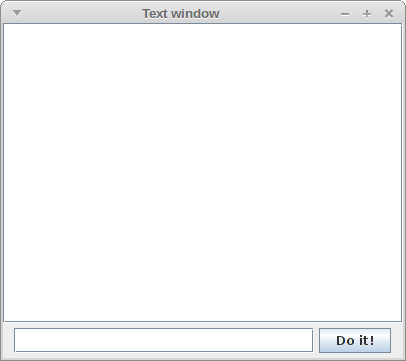
\includegraphics[scale=0.4]{res/gui_empty.png}
\end{frame}

\begin{frame}[fragile]{Hello World}
	\begin{lstlisting}
	import simple_gui.*;

	public class Example {

	    public static void main(String[] args) {
		
	        TextWindow window = new TextWindow();
	        
	        window.addOutputLine("Hello World!");
	        window.addOutputLine("");
	        window.addOutputLine("I am a Window.");
	    }
	}	
	\end{lstlisting}
\end{frame}

\begin{frame}{Hello World - Screenshot}
	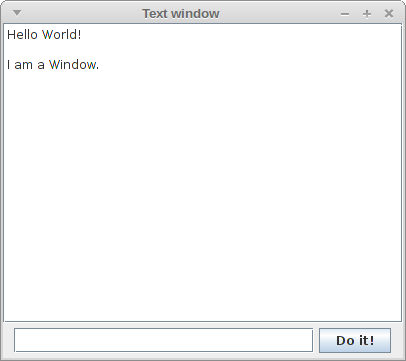
\includegraphics[scale=0.4]{res/gui_textlines.png}
\end{frame}

\subsection{Input}
\begin{frame}[fragile]{Input - Processing - Output - Loop}
	\begin{lstlisting}
	public static void main(String[] args) {
		
	    TextWindow window = new TextWindow();
	    
	    while(true) {
	        if (window.isInputAvailable()) {
	            // input:
	            String str = window.getNextInputLine();
	            // processing:
	            str = "user: " + str;
	            // output:
	            window.addOutputLine(str);
	        }	    
	    }
	}	
	\end{lstlisting}
\end{frame}

\begin{frame}{}
	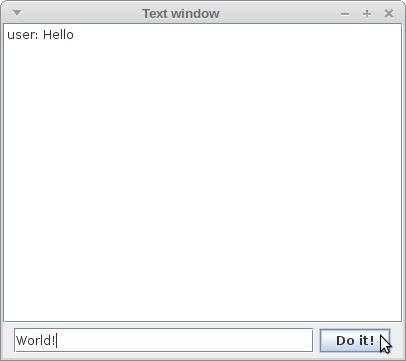
\includegraphics[scale=0.4]{res/gui_input.png}\\
	\footnotesize{During the second input. \\First input was \emph{Hello}. Second input will be \emph{World!}.}
\end{frame}

\begin{frame}[fragile]{Exit the Program}
	The \texttt{while(true)} statement implies the program will run forever. \\
	So you need a way to exit the program.
	\begin{lstlisting}
	while(true) {
	    if (window.isInputAvailable()) {
	        // input:
	        String str = window.getNextInputLine();
	        // processing:
	        if (str.compareTo("exit") == 0) {
	            window.close();
	            return;
	        }
	        str = "user: " + str;
	        // output:
	        window.addOutputLine(str);
	    }	    
	}
	\end{lstlisting}
\end{frame}

\subsection{Example ButtonWindow}
\begin{frame}[fragile]{Buttons}
	\begin{lstlisting}
	import simple_gui.*;

	public class ButtonTest {

	    public static void main(String[] args) {
		
	        // make a new window with 1 x 3 buttons
	        ButtonWindow window = new ButtonWindow(1, 3);
	    }
	}	
	\end{lstlisting}
\end{frame}

\begin{frame}{Buttons - Screenshot}
	We build a window with three buttons which have no function.
	\vfill
	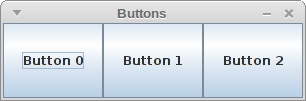
\includegraphics[scale=0.4]{res/gui_buttons.png}
\end{frame}

%TODO maybe add graphic explaining this procedure
\begin{frame}{ButtonWindow}
	The Javadoc says \texttt{configureButton(int buttonNumber, ButtonConfiguration config)}
	adds some configuration to the button.
	\vfill
	\emph{ButtonConfiguration} is an Interface that describes two methods:
	\begin{itemize}
		\item \texttt{String getButtonText()}
		\item \texttt{void onClickAction()}
	\end{itemize}
	\vfill
	We have to write a class that implements \emph{ButtonConfiguration} and pass an 
	instance to the method \texttt{configureButton(\dots)}. \\
	The configured button will be named with the String the method \emph{getButtonText()} will return.
	A clicked configured button will call the method \emph{onClickAction()}.
\end{frame}

\begin{frame}[fragile]{CloseButton}
	\begin{lstlisting}[basicstyle=\ttfamily\scriptsize, escapechar=!]
	import simple_gui.*;

	public class CloseButton implements ButtonConfiguration {

	    @Override
	    public String getButtonText() {
	        return "Close";
	    }

	    @Override
	    public void onClickAction() {
	        // implementation follows
	    }
	}	
	\end{lstlisting}
\end{frame}

\begin{frame}[fragile]{CloseButton - Test}
	\begin{lstlisting}
	import simple_gui.*;

	public class ButtonTest {

	    public static void main(String[] args) {
		
	        // make a new window with 1 x 3 buttons
	        ButtonWindow window = new ButtonWindow(1, 3);
	        
	        // the numeration starts with 0
	        // so the right button is no. 2
	        window.configureButton(2, new CloseButton());
	    }
	}	
	\end{lstlisting}
\end{frame}

\begin{frame}{CloseButton - Screenshot}
	The button is successfully renamed.
	\vfill
	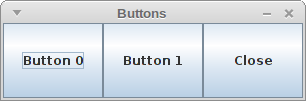
\includegraphics[scale=0.4]{res/gui_close.png}
\end{frame}

\begin{frame}[fragile]{CloseButton - onClickAction()}
	The method \texttt{window.close()} closes the window. 
	Unfortunately the class \emph{CloseButton} can not access the reference \texttt{window}.
	\begin{lstlisting}[basicstyle=\ttfamily\scriptsize, escapechar=!]
	@Override
	public String getButtonText() {
	    return "Close";
	}

	@Override
	public void onClickAction() {
	    // ...
	}
	\end{lstlisting}
\end{frame}

\begin{frame}[fragile]{CloseButton - onClickAction()}
	The class receives the reference through the constructor.
	\begin{lstlisting}[basicstyle=\ttfamily\scriptsize, escapechar=!]
	private ButtonWindow window;
	
	public CloseButton(ButtonWindow window) {
	    this.window = window;
	}
	
	@Override
	public String getButtonText() {
	    return "Close";
	}

	@Override
	public void onClickAction() {
	    this.window.close();
	}
	\end{lstlisting}
\end{frame}

\begin{frame}[fragile]{CloseButton - Final Test}
	\begin{lstlisting}[basicstyle=\ttfamily\scriptsize]
	import simple_gui.*;

	public class ButtonTest {

	    public static void main(String[] args) {
		
	        // make a new window with 1 x 3 buttons
	        ButtonWindow window = new ButtonWindow(1, 3);
	        
	        // pass the reference window as an argument
	        window.configureButton(2, new CloseButton(window));
	    }
	}	
	\end{lstlisting}
\end{frame}

\section{Abstract}
\subsection{Abstract}
\begin{frame}[fragile]{Abstract Class}
	The keyword \textbf{abstract} denotes an abstract class.
	\vfill
	\begin{lstlisting}
	public abstract class AbstractExample {
	
	}	
	\end{lstlisting}
	\vfill
	Like an interface you can not create objects from an abstract class.\\
	Abstract classes can extend other abstract classes and can implement interfaces.\\
	Abstract classes can be extended by normal and abstract classes.
\end{frame}

\begin{frame}[fragile]{Methods}
	An abstract class may has concrete methods and may has abstract methods.
	\begin{lstlisting}
	public abstract class AbstractExample {
	
	    public void printHello() {
	        System.out.println("Hello");	    
	    }
	    
	    public abstract String getName();
	}	
	\end{lstlisting}
	An abstract method forces the class to be abstract as well. \\
	\emph{Methods in an interface are also abstract but not denoted as such.}
\end{frame}

\begin{frame}[fragile]{Subclasses}
	The subclass has to implement abstract methods or has to be abstract as well.
	All concrete methods will be regular inherited.
	\begin{lstlisting}[escapechar=!]
	public class Example extends AbstractExample {
	    
	    @Override
	    public String getName() {
	        return "Example";	    
	    }
	}	
	\end{lstlisting}
\end{frame}

%TODO more text
\begin{frame}{Why using Abstract?}
	Abstract classes are used to minimize similar code in related classes.
\end{frame}

\subsection{Example AbstractButton}
\begin{frame}[fragile]{AbstractButton}
	\begin{lstlisting}[basicstyle=\ttfamily\scriptsize, escapechar=!]
	import simple_gui.*;

	public abstract class AbstractButton implements ButtonConfiguration {
	
	    protected ButtonWindow window;
	    private String label;
	
	    public AbstractButton(ButtonWindow window, String label) {
	        this.window = window;
	        this.label = label;
	    }

	    @Override
	    public String getButtonText() {
	        return label;
	    }
	}	
	\end{lstlisting}
\end{frame}

\begin{frame}[fragile]{CloseButton}
	\begin{lstlisting}[basicstyle=\ttfamily\scriptsize, escapechar=!]
	import simple_gui.*;
	
	public class CloseButton extends AbstractButton {
	
	    public CloseButton(ButtonWindow window, String label) {
	        super(window, label);
	    }

	    @Override
	    public void onClickAction() {
	        this.window.close();
	    }
	}	
	\end{lstlisting}
\end{frame}

\begin{frame}[fragile]{Test}
	\begin{lstlisting}[basicstyle=\ttfamily\scriptsize]
	import simple_gui.*;

	public class ButtonTest {

	    public static void main(String[] args) {
		
	        // make a new window with 1 x 3 buttons
	        ButtonWindow window = new ButtonWindow(1, 3);
	        
	        window.configureButton(2, 
	            new CloseButton(window, "Close"));
	    }
	}	
	\end{lstlisting}
\end{frame}

%TODO Overview
%\begin{frame}{Abstract Class vs. Interface}
%
%\end{frame}

%TODO Common Errors
%\begin{frame}{Static vs. Abstract Methods}
%	Do not mix up statitic and abstract methods.
%\end{frame}
\end{document}